%!TeX root = sensor_mcu
\documentclass[../main.tex]{subfiles}

\begin{document}
    \section{Current sensor and MCU}
    \begin{figure}[!h]
        \centerline{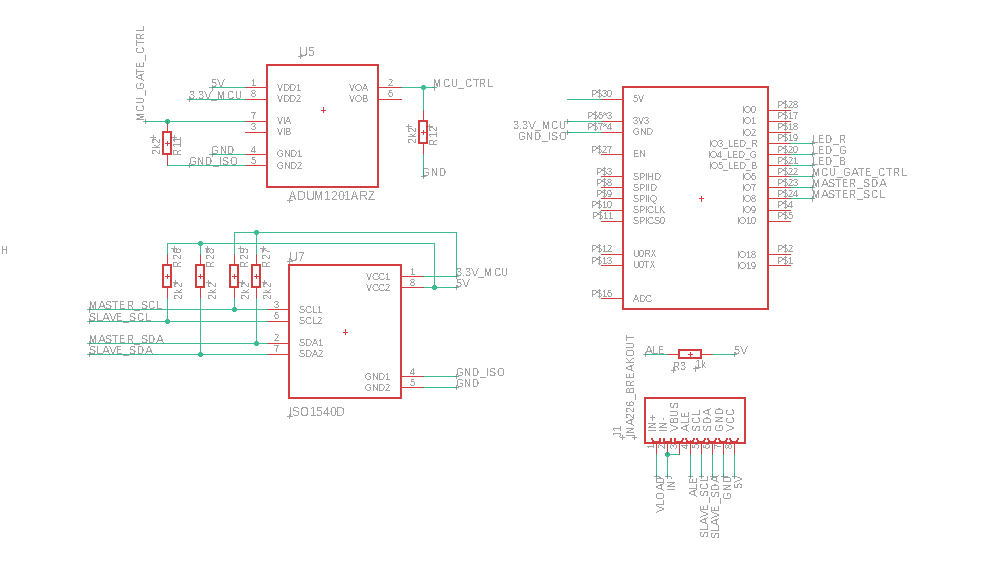
\includegraphics[width=\linewidth]{media/sensor_mcu_schematic.png}}
        \caption{Current sensor, MCU and signal isolation ICs schematic.}
        \label{fig:latch_circuit_schematic}
    \end{figure}
    In this section, the features of the current sensor and the MCU is discussed.

    \pagebreak
    \subsection{Current sensor INA226}
    \justify
    The current sensor is a sensor board centering around the IC INA226 from Texas Instruments Inc. \cite{INA226}. The followings are some note-worthy features of the device:
    \begin{itemize}
        \item All-in-one solution for power monitor. The IC provides direct readout of bus voltage, current, and power (calculated from the measured values). It is also suitable for both high-side and low-side measurement because the bus voltage is measured separately by pin VBUS.
        \item Shunt-based, wide shunt measurement range $\lbrack-81.9175mV, 81.92mV\rbrack$, and adequate ADC resolution of 16bits. These allow for a flexible setup without sacrificing accuracy. In particular, using a $0.004$ shunt, a resolution of $2.5\mu V / R_{shunt} = 625 \mu A$, and a measuring range of $\lbrack-20.5A, 20.5A\rbrack$ are achieved.
        \item I2C interface allowing up to 4 devices of the same type, and average filter programming.
        \item Alert function which can be programmed to control the ALE pin based on voltage or current or power exceeding a programmable limit.
    \end{itemize}

    \justify
    In this project, the INA226 sensor board is setup as follow:
    \begin{itemize}
        \item To avoid ground offset as explained in previous section, INA226 is set up as a high-side measurement unit.
        \item Bus voltage is measured at the negative terminal of the shunt, measuring the voltage drop across the load. This means the VBUS and IN- pins are shorted.
        \item The alert function is programmed to send a positive pulse when power exceeds a set limit.
    \end{itemize} 

    \pagebreak
    \subsection{ESP32-C3 development board}

    \justify
    The ESP32-C3 development board is centered around the ESP-C3-32S from Shenzhen Ai-Thinker Technology Co., Ltd. \cite{ESP32}. The MCU is a single-core $3.3V$ processor. The board is shipped with the following peripherals:
    \begin{itemize}
        \item UART-to-USB converter.
        \item LDO converter to power the board from sources above $5V$ or from the USB.
        \item On-board antenna for WiFi connectivity.
        \item On-board RGB LED (tied to GPIO3, GPIO4, GPIO5) which is programmed to show errors the device is encountering.
    \end{itemize}

    \justify
    The GPIO of the board is used as follows:
    \begin{itemize}
        \item GPIO4 and GPIO5 are used for showing errors the device is encountering.
        \item GPIO7 and GPIO8 are SDA and SCL respectively.
        \item GPIO6 for MCU\_CTRL signal in the latch circuit.
    \end{itemize}

    \justify
    The board is powered by the isolated 5V rail discussed in previous section. To integrate the board with other components such as the latch circuit and INA226, a digital isolator IC and an I2C isolator IC are required. 
    \begin{itemize}
        \item The digital isolator chosen is the ADUM3201ARZ from Analog Devices Inc. \cite{ADUM3201} is chosen. This IC uses transformer-based iCoupler technology instead of the traditional optocoupler which eliminates the need for external driver.
        \item The I2C isolator chosen is the ISO1540 from Texas Instruments Inc. \cite{ISO1540}.
    \end{itemize}
    

\end{document}